\documentclass[tikz,border=0pt]{standalone}
\usepackage[T1]{fontenc}
\usepackage{lmodern,amsmath,amssymb,graphicx}
\usetikzlibrary{arrows.meta,calc,positioning}
\definecolor{blue}{HTML}{0072B2}
\definecolor{orange}{HTML}{D55E00}
\definecolor{ink}{HTML}{25313B}
\renewcommand{\familydefault}{\sfdefault}
\begin{document}
\begin{tikzpicture}[x=1cm,y=1cm,font=\sffamily\fontsize{7}{8.5}\selectfont,>=Stealth,
 box/.style={draw=ink!35,fill=white,rounded corners=2pt,align=center,text width=3.8cm,minimum height=1.05cm,inner sep=5pt,line width=.55pt},
 arr/.style={->,line width=.65pt,draw=ink!65}]
 \path[use as bounding box] (0,0) rectangle (18,12.4);
 \node[anchor=west,font=\sffamily\fontsize{7}{8.5}\selectfont\bfseries] at (.25,12) {a};
 \node[anchor=west,font=\sffamily\fontsize{7}{8.5}\selectfont\bfseries] at (.7,12) {The same sender noise produces different patterns of receiving noise};
 \node[box,fill=blue!4] (source) at (2.65,10.35) {Hold actual sender probabilities and credibility scores fixed.\\[4pt]Community innovations $\varepsilon$\\$\operatorname{Cov}(\varepsilon\mid S)=\operatorname{diag}(v_c)$};
 \node[box,fill=blue!4,text width=3.65cm,minimum height=.8cm] (ring) at (9,11.05) {Local routing: $C=B$};
 \node[box,fill=orange!4,text width=3.65cm,minimum height=.8cm] (broadcast) at (9,9.55) {Common routing: $C=\mathbf1\omega^\top$};
 \node[box,fill=ink!3] (receive) at (15.35,10.35) {Receiving innovation $\eta=C\varepsilon$\\[4pt]$\operatorname{Cov}(\eta\mid S)$\\$=C\operatorname{diag}(v_c)C^\top$};
 \draw[draw=ink!65,line width=.65pt] (source.east)--(5.35,10.35);
 \draw[arr] (5.35,10.35)|-(ring.west);
 \draw[arr] (5.35,10.35)|-(broadcast.west);
 \draw[draw=ink!65,line width=.65pt] (ring.east)--(12.65,11.05)--(12.65,9.55)--(broadcast.east);
 \draw[arr] (12.65,10.35)--(receive.west);
 \node[align=center,text width=16.7cm] at (9,8.42) {A common broadcast reduces each community's marginal noise here, while making receiving noise perfectly shared.\\[3pt]This is a conditional routing comparison, with no recomputation of choices and no new simulated trajectories.};
 \draw[ink!16,line width=.5pt] (.4,7.75)--(17.6,7.75);
 \node[anchor=south west,inner sep=0pt] at (0,.15) {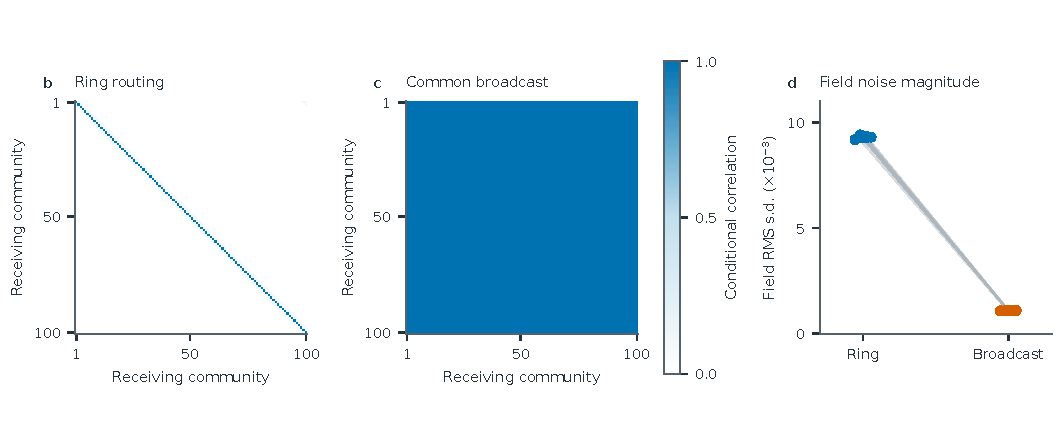
\includegraphics[width=18cm]{supp10_noise_panels.pdf}};
\end{tikzpicture}
\end{document}
